\documentclass[a4paper]{article}
\usepackage[MeX]{english}
\usepackage{hyperref}
 \hypersetup{pdfborder={0 0 0}}
\usepackage[utf8x]{inputenc}
\usepackage{lastpage}
\usepackage{fancyhdr}
\usepackage{rotating}
\usepackage{graphicx}
\graphicspath{{./img/}}
\DeclareGraphicsExtensions{.pdf,.png,.jpg}


\pagestyle{fancy}
\fancyhead{}
\fancyfoot{}

\lhead{Little Benchmark: HDD}
\rhead{Read Me}
\cfoot{page \thepage/\pageref{LastPage}}

\begin{document}
\title{Little Benchmark: HDD  \LaTeX2}
\author{Author: Łukasz Buśko
\\License: General Public Licens
\\Home:  \href{https://str0g.wordpress.com}{https://str0g.wordpress.com}
%\\email:\href{mailto:buskol.waw.pl@gmail.com}{buskol.waw.pl@gmail.com}
\\Copyright \copyright 2010-2011 Łukasz Buśko\\
\date{\today} Version.: 1.1.2}
\maketitle
\newpage
\tableofcontents
\newpage
\hypertarget{License}{
\section{License}
\label{License}\index{License@{License}}
}
This program is free software; you can redistribute it and/or modify
it under the terms of the GNU General Public License as published by
the Free Software Foundation; either version 2 of the License, or
(at your option) any later version.\\
This program is distributed in the hope that it will be useful,
but WITHOUT ANY WARRANTY; without even the implied warranty of
MERCHANTABILITY or FITNESS FOR A PARTICULAR PURPOSE.  See the
GNU General Public License for more details.\\
You should have received a copy of the GNU General Public License
along with this program; if not, write to the Free Software
Foundation, Inc., 675 Mass Ave, Cambridge, MA 02139, USA.
    
\section{Requirements}
Operating system: Linux, Windows XP or newer\\
Library.:libboost 1.40 , libcrypto++ 5.6.0-5
\section{Features}
\begin{itemized}
\item Portability (not tested yet)
\item Multi threading for controllers and NCQ tests
\item Test read by 1 character and stream
\item Test read by chunk useful for server disk drivers speciality if test in multi threading (no implemented yet)
\item Read files are being validated with sha512 hash sum after read test in order to check if we read what we supposed to read
\item Nanoseconds precision
\item Human readable output (style of log, formatted text, or xml(N/A) file)
\item Easy and fully customizable by command line or configuration file
\item Tests designed for hybrid drives(currently not enabled)
\item Free of charge but don't forget to appreciate my job by \href{http://str0g.wordpress.com/about/}{\underline{donation}}
\end{itemized}

\newpage
\hypertarget{Howdoesitwork}{
\section{How does it work}
\label{Howdoesitwork}\index{Howdoesitwork@{How does it work}}
}
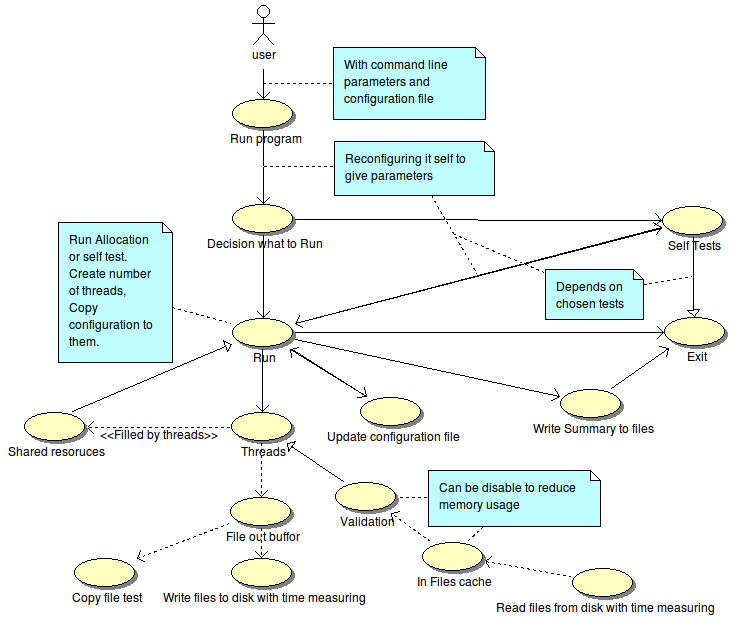
\includegraphics[scale=0.55]{short_how_it_works_diagram}
\caption{Simplified use case diagram}
\label{UseCaseDiagram}

\newpage
\hypertarget{Installation}{
\section{Installation}
\label{Installation}\index{Installation@{Installation}}
}

\subsection{Package}
Binaries and source can be downloaded from:
\begin{description}
\item \href{http://github.com/str0g/LittleBenchmark/tree/master/HDD/Release}{Git Not uploaded yet}
\item \href{https://subversion.assembla.com/svn/littlebenchmark-hdd/}{SVN Not uploaded yet}
\end{description}

\subsection{Linux}

\subsubsection{From Repository(not uploaded yet)}
Open terminal and copy content:
\begin{verbatim}
sudo add-apt-repository ppa:buskol-waw-pl/littlebenchmark-hdd
sudo apt-get update
sudo apt-get install littlebenchmark-hdd
\end{verbatim}

\subsubsection{From source}
Open terminal:\\
\$ cd \ldots/Littel\_Benchmark/HDD\\
\$ ./configure\\
\$ make \&\& make test \&\& make install \&\& make clean\\
\subsection{Windows}
Windows port will be done latter.

\subsubsection{From source}
What is needed to compile from source: (Working on it\ldots)
\begin{itemize}
\item [ \href{http://sourceforge.net/projects/mingw/files/Automated\%20MinGW\%20Installer/mingw-get-inst/mingw-get-inst-20100909/mingw-get-inst-20100909.exe/download/}{\textbf{MiniGw gcc}} ] Compiler to make things possible.
\item [ \href{http://www.codeblocks.org/}{\textbf{CodeBlocks}} ] IDE.
\item [ \href{http://sourceforge.net/projects/boost/files/boost/1.41.0/boost_1_41_0.7z/download}{\textbf{Boost library}} ] This Library takes care about porting issues between Linux and Windows.
\item [ \href{http://www.cryptopp.com/}{\textbf{Crypto++}} ] Cryptographic library for file validation.
%\item [ \href{http://qt.nokia.com/downloads/}{\textbf{Qt4 sdk}} ] To compile cryptopp.
\item [ \href{http://notepad-plus-plus.org/}{\textbf{Notpad++}} ] For file editing with out blowing encoding.
\end{itemize}
Set up Compiler:\\
Check download C++ , C - objective, msys* stuff \\
After installation successful end.\\
Press button with windows logo + break/pause got to environment variable\\
Edit Path, add \begin{verbatim}  ";C:\MiniGw\bin;C:\MinGW\msys\1.0\bin" 
\end{verbatim}

Set up boost:\\
open command line\\
ctrl + r type cmd
\begin{verbatim} 
cd boost_dir/
boostrap.bat
\end{verbatim}
Insert to project.config.jam "using gcc ;"
\begin{verbatim} 
bjam --tool-set=gcc --build-dir=boost-build --build-type=complete stage release --without-python
bjam --build-dir=boost-build --toolset=gcc install --without-python
\end{verbatim}

%Set up Cryptopp:\\
%Unpack to C:\\
%With make only: (does not work)\\
%\begin{verbatim} 
%cd C:/cryptopp561
%make
%\end{verbatim}
%With qt4: (does not work)\\
%start\rightarrow All Programs\rightarrow Qt sdk\ldots \rightarrow Qt Command prompt
%\begin{verbatim} 
%cd C:/cryptopp561
%qmake -project
%\end{verbatim}
%Edit the cryptopp561.pro with notpad++\\
%change TEMPLATE = app to TEMPLATE = lib\\
%add a lines\\ 
%LIBS += -lws2\_32 \\
%CONFIG += console.\\
%
%type the following commands at the Qt command line:
%\begin{verbatim}
%qmake
%mingw32-make all
%\end{verbatim}
%%now we should have files named libcryptopp552.a and cryptopp552.dll in directories C:\cryptopp552\release and C:\cryptopp552\debug
%
%
%Compile Project with make:\\
Compile Project with Codeblocks:
Settings->Global Variables->New\\
Name it boost
\begin{verbatim}
base bath C:\boost
include bath C:\Boost\include\boost-1_41
lib bath C:\boost
\end{verbatim}
%Next New variable cryptopp
%\begin{verbatim}
%base bath C:\cryptopp
%include bath C:\Boost\include\boost-1_41
%lib bath C:\boost
%\end{verbatim}
%\href{http://www.perl.org/get.html}{Perl for Windows (Automake requirement)}
%\href{http://gnuwin32.sourceforge.net/packages/automake.htm}{Automake for Windows}
%Then install Perl and Automake
%\begin{verbatim}
%
%cd ...\Little_Benchmark\HDD
%configure
%make
%make test
%make install
%make clean
%\end{verbatim}
\hypertarget{Configuration}{
\section{Configuration}
\label{Configuration}\index{Configuration@{Configuration}}
}
Please Run binary with -M option to set max string and char size in order to avoid memory allocation error.

To get information what options can be specified run program with -h option.
\subsection{Linux}
Configuration file is going to be created in \$HOME/.littlebenchmark/hdd
\subsection{Windows}
Configuration file is going to be created in:\\
Windows 7 / Vista: ROOT FILE SYSTEM/USER/APPData/Local/.littlebenchmark/hdd\\
XP: ROOT FILE SYSTEM/USER/Local Settings/Application Data/.littlebenchmark/hdd\\

\newpage
\hypertarget{KnownIssues}{
\section{Known issues}
\label{KnownIssues}\index{KnownIssues@{Known issues}}
}

{\bf Before appalling any solution in Linux run terminal session ctrl+alt+F1 and login with root privilege, in order to avoid any sort of problems!\\
After applying solution check if you can login in other terminal session and unlock lock screen.\\ \\
}
{\bf Before applying any solution on WinCrap pray and backup important data.
}

\begin{description}
\item [\bf{Memory leak}] 32 records lost when running with -M\\ Solution unknown: Lost is in static allocated memory.
\item [\bf{Strange Log Output}] Example: \begin{verbatim}
Min:1e+09s
Max:[Failed to measure: time difference to small]
Avg:-nans
\end{verbatim}\\
Memory allocation failed or your hard drive for given data is immeasurable fast :-)

\item [{\bf Linux}] Memory leak caused by bug in {\itshape pwd.h} library
\marginpar{12 records in worst case scenario can take max 8192 bytes, libc-freeres won't do the job so please apply solution}
\begin{verbatim}
#include <pwd.h> /*12 records lost*/
struct passwd *pw;
\end{verbatim}
\\{\bf Solution:} line 7-9 word ``{\itshape compat}'' have to be replaced with ``{\itshape files}''
\begin{verbatim}
lukasz@lukasz-compal:~$ cat -n /etc/nsswitch.conf 
     1	# /etc/nsswitch.conf
     2	#
     3	# Example configuration of GNU Name Service Switch functionality.
     4	# If you have the `glibc-doc-reference' and `info' packages installed, try:
     5	# `info libc "Name Service Switch"' for information about this file.
     6	
     7	passwd:         compat
     8	group:          compat
     9	shadow:         compat
    10	
    11	hosts:          files mdns4_minimal [NOTFOUND=return] dns mdns4
    12	networks:       files
    13	
    14	protocols:      db files
    15	services:       db files
    16	ethers:         db files
    17	rpc:            db files
    18	
    19	netgroup:       nis
\end{verbatim}

\end{description}

\newpages
\end{document}
